\chapter{Introduction}
\minitoc% Creating an actual minitoc

\par In one sentence, my PhD focus on extract, quantify and \textit{transfer} of \textit{styles} or \textit{personas}, isolated from a task, using deep neural networks.

\section{What is a style?}\label{sec:style}
  \par Style is generically defined in Merriam-Webster dictionary (figure \ref{fig:style_def_webster}).

  \begin{figure}[!htbp]
    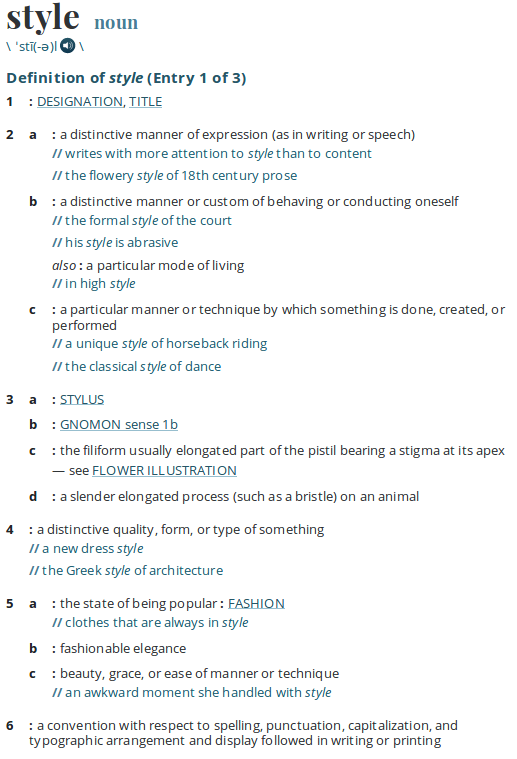
\includegraphics[scale=0.6]{./images/introduction/style_def_webster.png}
    \caption{Definition of style in Merriam-Webster dictionary}
    \label{fig:style_def_webster}
  \end{figure}

  \par In general, it is defined as \textit{the manner of doing things}\citep{gallaher1992individual}. To get more sense of what style is, it is better to give some examples first, to get an idea about what we are dealing with.
  \begin{itemize}
    \item When we say the word "seriously?". Depending on the manner we say it, it will carry different meaning (sarcastic or surprise for example). One word, two different manners to say it.
    \item Handwriting: You can the same the letter (the task), but with multiple typefaces (the style) (figure \ref{fig:different_fonts}).
    \item A movie setting: the script is provided to the actor. There are, however, many ways for the actor to perform what is written in the script, in order to convey different messages/experiences to the audience.
  \end{itemize}

  \begin{figure}[!htbp]
    \begin{center}
      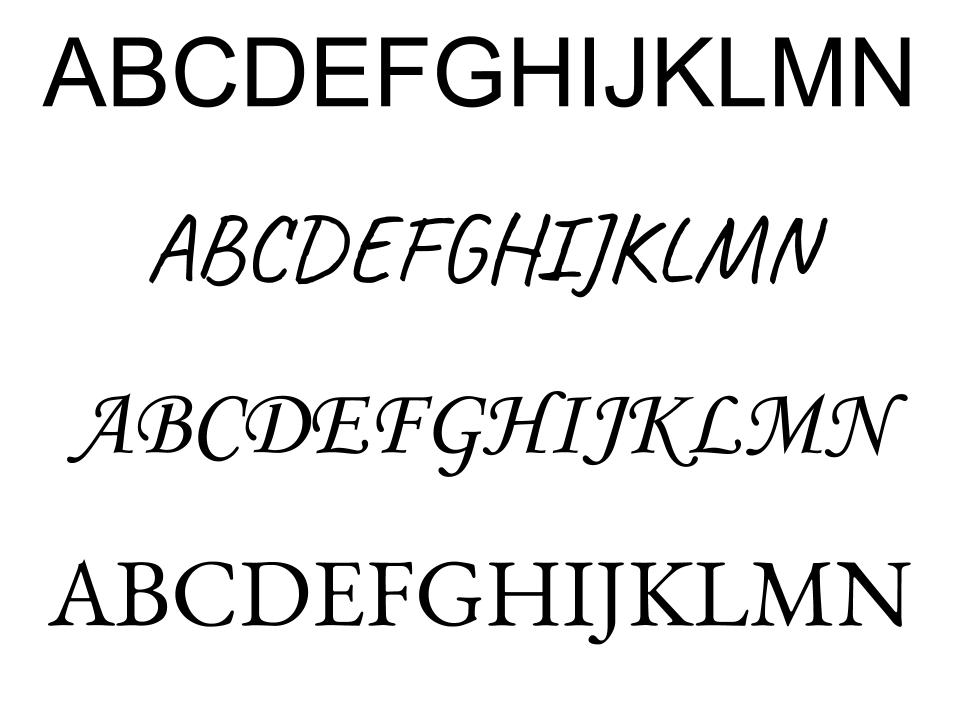
\includegraphics[scale=0.3]{./images/introduction/different_fonts.jpg}
    \end{center}
    \caption{Multiple styles (different typefaces) for the same letters.}
    \label{fig:different_fonts}
  \end{figure}

  In these two examples, we see a basic structure:
  \begin{itemize}
    \item A fixed part: the word to be said, or the letter identity. We will call this the \textit{content}.
    \item A variable part: the manner we say the word, or the manner we write the letter. We will call this the \textit{style}.
    \item Together, a style and a content forms a \textit{task}.
  \end{itemize}

  \par The mention of styles is quite a lot in the literature in multiple domains, for example:
  \begin{itemize}
    \item \textbf{Speech synthesis}: \citep{tachibana2004hmm} defines speaking style in a high-level manner, in terms of emotions expressed by the speaker, like 'joy', 'sad', or the interpolation between them, when reading a text. \citep{wang2018style} looks at the speech style in a more detailed manner, considering different aspects of speech prosody, like the paralinguistic information, intonation and stress.
    \item \textbf{Car driving}: there are multiple ways to categorize the different driving styles. It can be based on the safety aspect \citep{johnson2011driving}, the aggressiveness of the maneuver \citep{dorr2014online,xu2015establishing}, the impact on fuel consumption \citep{manzoni2010driving,neubauer2013accounting}. Many other identification basis for driving styles are summarized nicely in \citep{martinez2017driving}.
    \item \textbf{Handwriting}: handwriting can be offline (the final image of the letter) or online (recording the movement of the pen/drawing tool). Depending on which one considered, the style profile can change. Figure \ref{fig:different_fonts} is an example of different offline styles (the typefaces). But when we consider the online aspect of the drawing, we can see different aspects, like in figure \ref{fig:online_handwriting_styles}, where we see that the same drawing can be in clockwise or counterclockwise direction (we will expand more on this point in chapter \ref{ch:framework_sec:styleperletter}).
  \end{itemize}

  \begin{figure}[!htbp]
    \centering
    \begin{subfigure}[tb]{0.45\textwidth}
        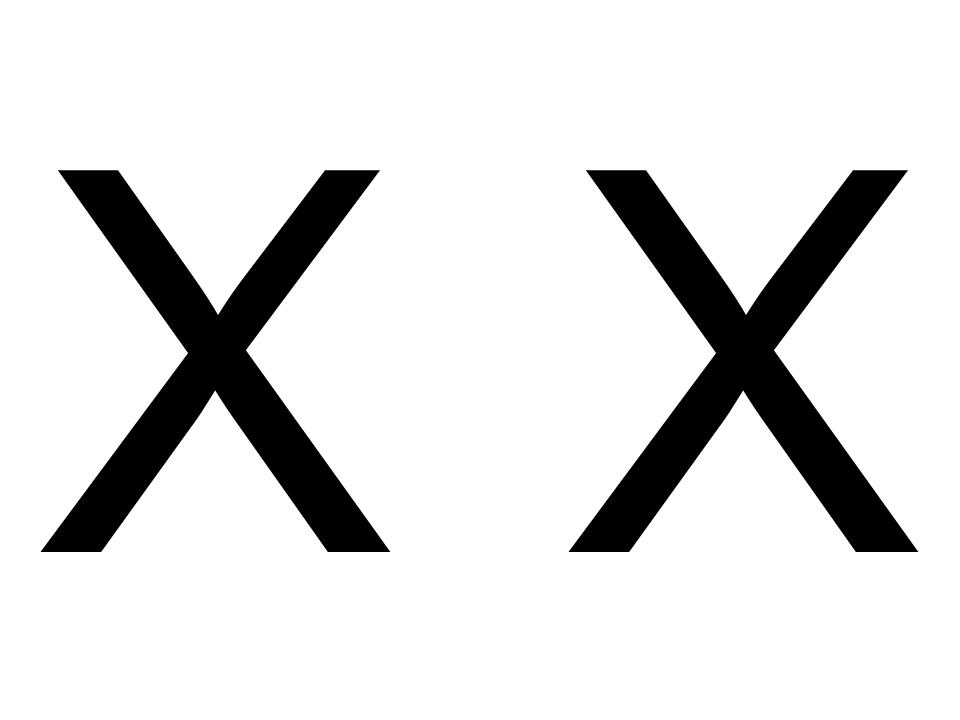
\includegraphics[width=\textwidth]{images/introduction/DIFFERENCE_IN_STYLE_PERCEPTION_1.jpg}
        \caption{Offline drawing}
    \end{subfigure}

    \begin{subfigure}[tb]{0.45\textwidth}
        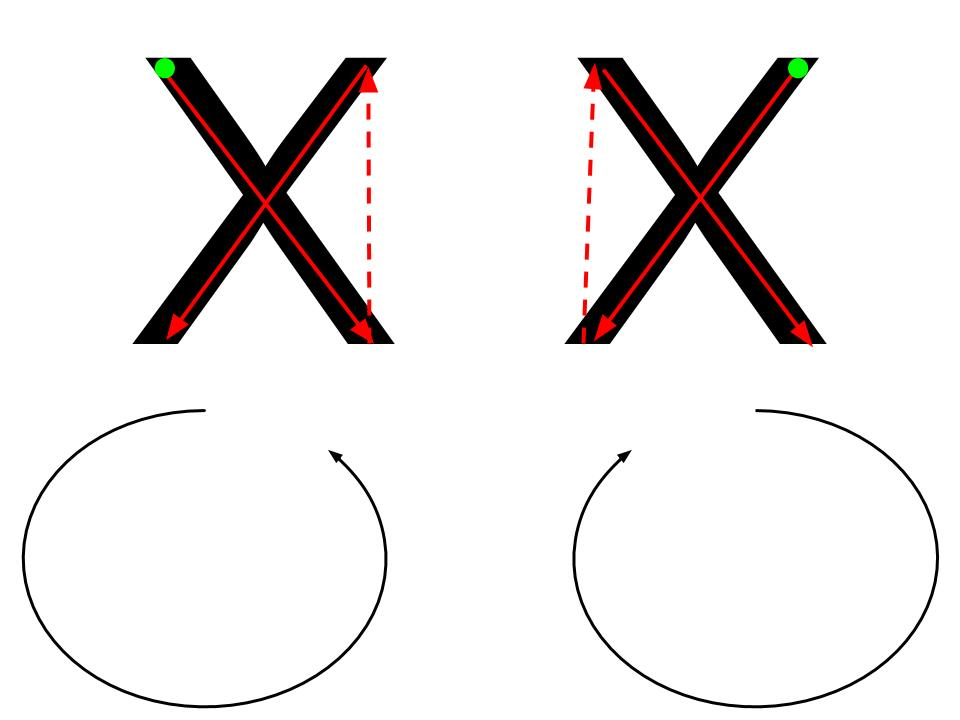
\includegraphics[width=\textwidth]{images/introduction/DIFFERENCE_IN_STYLE_PERCEPTION_2.jpg}
        \caption{Online drawing}
    \end{subfigure}
    \caption{Example for style in case of online handwriting. Although both examples looks the same when we look at it in the offline mode (the final drawing), they are quite different when we consider the online aspect (the dynamics of the pen when drawing them). In this case, the starting point and the direction of drawing (clockwise or counterclockwise) are different. The solid line indicate a stroke, and the dotted line indicate an air stroke (the transition of the pen in the air between two strokes). The green dot is the starting point.}
    \label{fig:online_handwriting_styles}
  \end{figure}

  \par One thing can be seen here: there is no one definition for styles. It depends on the way you look at the problem, and the aspect of interest, and the way we look at the problem. This leads to an important characteristic of \textit{styles}, that it is an ill-defined concept. We know that \textit{styles} are rich in information and important in communication between humans. They are needed in order to convey meaning. As noted in \citep{taylor2009text} -- in the context of speech synthesis --, a proper rendering of styles affects the overall perception. However, we can not completely remove the ambiguity in this definition.

% Talk about style in images, speech, handwriting, driving,...etc. Also, distinguish between static and temporal styles.
% \setlist{nolistsep}\begin{itemize}[noitemsep]
%     \item What is a task? what is a style? how both combine to give us an experience?
%     \item Possible scenarios: images, speech, handwriting, autonomous driving
%     \item Style perception depends on 'how you look at it' (the light - angle of view -, body - task - and shadow - the resulting style - example) (cooking rice: no spices or with curcuma. perception: color? taste?) (handwriting: online styles? offline style?). Then end up with the conclusion that styles are ill-defined.
% \end{itemize}


% \section{Why studying styles?}
% \setlist{nolistsep}\begin{itemize}[noitemsep]
%     \item Shortcoming of applying machine learning methods -- average over previous scenarios, doesn't consider styles in advance --.
%     \item HRI example: the need for personalization to enhance the interaction experience.
%     \item Speech example: different utterances change the perceived message
% \end{itemize}



\section{What is the objective of the this whole project?}
\par Our long-term objective is to enable our humanoid iCub robot Nina \ref{fig:nina_robot}, to have a exhibit personalized behavior suitable for the person interacting with it. This will enhance the user experience, and will allow for a more natural interaction with the robot. It is shown that a robot with exhibiting a personalized behavior is more likable acceptable by humans, and perceived as an intelligent entity \citep{churamani2017impact}. Humans have different preferences when interacting with each other, or interacting with the robot, and taking them into account does improve the quality of interaction, and the potential of success for the task \citep{kashi2018smooth}.

\par At the moment, we successfully used machine learning approaches in order to build models of human-robot interaction \citep{mihoub2016graphical,bailly:hal-01939223,nguyen:hal-01609535}. However, when using these models to generate behaviors, this behavior usually represents an average over the learned behaviors (which is expected). The goal is to learn models of styles, and use it to bias the models of interaction that we have, in order to generate more personalized behaviors.

\begin{figure}[!htbp]
  \begin{center}
    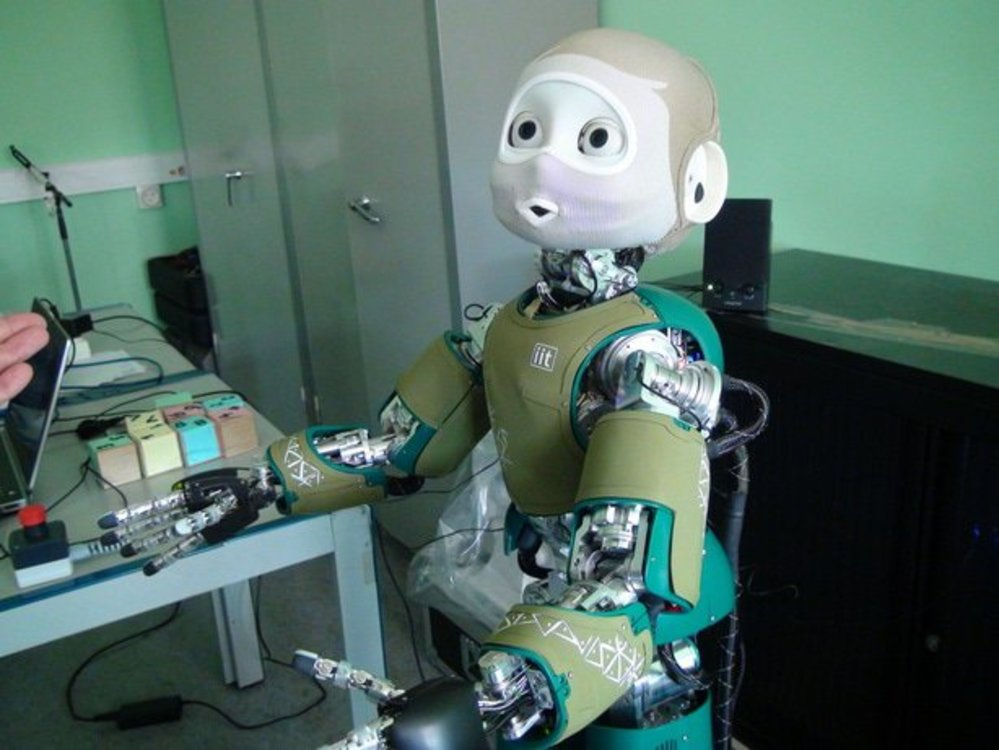
\includegraphics[scale=0.3]{./images/introduction/nina_robot.jpg}
  \end{center}
  \caption{The iCub humanoid robot (Nina).}
  \label{fig:nina_robot}
\end{figure}

\section{Why Handwriting?}
  \par As mentioned earlier, the final objective of this project is to extract and transfer styles in the context of human-robot interaction. What this has to do with handwriting?
  \par The usage of deep learning in HRI is still in its infancy, mainly because of the lack of datasets. The issue is not collecting the data (there are many small open-source datasets available online), but having a unified set of objective and platforms for HRI, which is not an easy challenge. We envision that this problem will be resolved, as there is a growing interest in the community to address it.

  \par Thus come handwriting. We use it as a proxy platform to understand, build and test different approaches to use deep learning. It has many advantages to make it a good proxy, including:
    \begin{itemize}
    \item Availability of dataset: several excellent datasets already exist, with large quantities of data.
    \item Diverse of tasks and styles: there are many tasks (letters) in handwriting, ranging from simple (like letter 'C') to complex (like letter 'E'), and the writers exhibit a diverse set of styles on the different tasks, making handwriting a good candidate to explore the problem of styles.
    \item Several style aspects are accessible to investigate visually, making it more accessible for in-depth analysis, and getting insight on how the model behaves.
    \item Several datasets provide information about the writers, like the age, handiness, gender and the origin. This data is interesting in some aspects of the style problem.
    \item We have a clear idea about the content of each task (the identify of the letter or the shape). Usually, the task is presented to us with the content and the style mixed together. How to disentangle the content from the style is an open question, and the fact the styles is an ill-defined problem makes it more ambiguous. With the assumption that we know the content, we can focus our effort on the styles problem\endnote{We will argue later that the task identity is not necessarily a good representation for the task content.}.
    \end{itemize}
  A disadvantage of handwriting is the lack of the \textit{interaction} aspect in handwriting.

\section{What is transfer learning? and why do we need it?}
\par We will discuss transfer learning in more detail in chapter \ref{ch:seat}, but for now, we want to motivate having this as one of the PhD objectives.

\par Transfer of knowledge deals with the problem of leveraging the knowledge learned from one task, to accelerate/improve the learning of a new task. This is a skill human do naturally, for example, if you learn Mathematics, and you want to learn physics, you can easily leverage the knowledge of Mathematics to bootstrap your learning of physics. This, intuitive as it seems, is not straightforward for machine learning models. A change in the distribution of the input to the model leads to significant degradation in the performance of the model \citep{shimodaira2000improving}.

\par Transfer learning is thus a field of machine learning, concerned with developing algorithms and procedures, to enable the transfer of knowledge between different tasks. So many techniques are available for transfer learning, but there is always a common assumption, that the transfer has the potential of success if the tasks are related (i.e., if there is common knowledge between the tasks), otherwise, a transfer learning can at best lead to no improvement, or even reduce the performance of the new model \citep{weiss2016survey}.

\par Why do we need transfer learning? We do not always have the advantage of large datasets on the tasks that we want. In many cases, the acquisition and/or the annotation of large dataset can be prohibitively expensive. A simple relevant example here is HRI: collecting large dataset on each scenario we want to learn is simply unfeasible, due to the huge time it takes, and the limitations/cost of the hardware. Thus, we need to be able to transfer the knowledge from the task where we have large amount of data, to a relevant task where we do not have this advantage (figure \ref{fig:illustrate_TL}).

\par What we want to achieve in this thesis is to transfer the styles between different tasks. We hypthosize that, when the tasks

\begin{figure}
  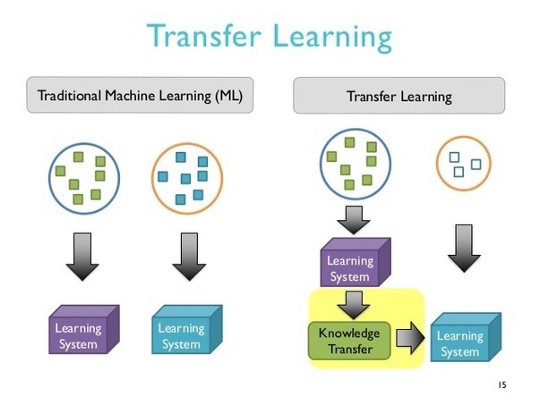
\includegraphics[scale=0.8]{./images/introduction/transfer_learning_illustration.jpeg}
  \caption{Illustration for a practical case of using transfer learning, where we have insufficient data on the new task, and we want to leverage the knowledge learned from another relevant task in order to learn the new task\endnote{Source of this image is \url{https://medium.com/data-science-101/transfer-learning-57ce3b98650}}.}
  \label{fig:illustrate_TL}
\end{figure}
\section{If we want transfer learning, why extracting styles?}
  \par interpretability is important for trust and debugging (use the arguments from the book)


\section{Contributions of this PhD}
\par In this manuscript, we discuss the different contribution of this PhD, addressing different aspects of the styles:
\begin{enumerate}
  \item
\end{enumerate}
Some informal contributions are: \textbf{not sure about this section}
\begin{enumerate}
  \item Definition of styles??
\end{enumerate}

\section{An overview of the manuscript}
\par The main contribution of the PhD is a thinking framework to study and observe styles, in the temporal case, using neural networks, while the task is defined beforehand. Through implementation, benchmarks and evaluation, and analysis of the networks performance (and sometimes its behavior), we seek to provide support to ground this framework, and our hypotheses about it.

\par The most general elements/components has been used in our study, in order not to couple the effect of more advanced/complicated items with our conclusions. This leaves a big room for further improvements and exploration as well.

\par Using machine learning as tool enables us to process large amount of data.

\section{Thesis outlines}
